% Software and tools used: Explain the software and tools you used for 
% your implementation. This could include programming languages, libraries, 
% frameworks, or any other tools that you found useful.
\section{Implementacja}

% Data preparation: Discuss the data preparation steps you took, 
% including data cleaning, feature selection, and data normalization. 
% Explain how you handled missing values and outliers, and any techniques 
% used to preprocess the data.
\subsection{Przygotowanie danych}

W celu stworzenia zbioru testowego i treningowego zbiór danych został podzielony
na dwie części, a poszczególne obserwacja zostały połączone w krótsze serie danych.
Reorganizacja danych została dokonana poprzez zastosowanie przesuwnego okna próbkującego
dane z krokiem 24 godzin. W ten sposób na każde 96 godzin obserwacji przypada 24 godziny predykcji
będące odczekiwanym wynikiem działania modelu. Próbkowanie zostało zastosowane z nakładaniem się,
co znaczy, że dane będące w jednym kroku wyjściem, w następnym kroku są używane jako dane wejściowe.

\begin{figure}[H]
    \centering
    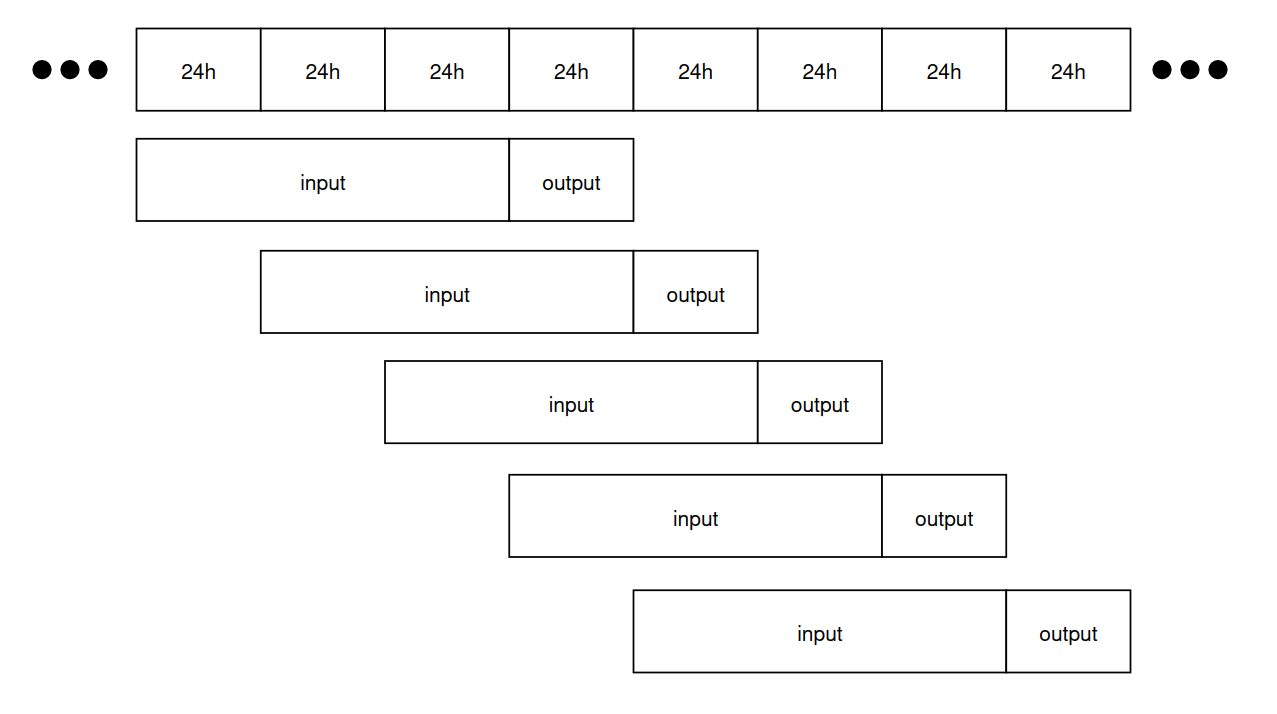
\includegraphics[width=\textwidth]{images/division.png}
    \caption{Sposób podziału zbioru danych na dane wejściowe i wyjściowe}
    \label{division}
\end{figure}


% Model development: Explain how you developed the models used for your 
% analysis. Discuss the algorithmic choices and parameter settings, 
% as well as any tuning or optimization steps.
\subsection{Zaprojektowanie modelu}

W celu znalezienie hiperparametrów zapewniających najlepszą dokładność modelu,
dwie metody przeszukiwania przestrzeni możliwych wartości zostały zastosowane:

\begin{itemize}
    \item Grid Search — działa poprzez wyczerpujące przeszukiwanie 
    przestrzeni dostępnych parametrów i wybiera hiperparametry maksymalizujące
    średnią dokładność z walidacji krzyżowej dokonanej na zbiorze treningowym.
    \item Halving Grid Search — zoptymalizowana czasowo wersja Grid Search
    przydzielająca początkowo ograniczone ilości zasobów (mniejszą ilość
    danych). W miarę ewaluacji algorytmu iteracyjnie pomniejszany jest zbiór
    rozważanych hiperparametrów, a najlepszy dobór ewaluowany jest na coraz większym
    zbiorze danych.
\end{itemize}

Niektóre z wykorzystanych modeli nie są przystosowane do przeprowadzania 
regresji z wielowymiarowym wyjściem, przez co konieczne jest stworzenie strategii,
w której dla każdy wymiar wyjściowy wymaga stworzenia osobnego modelu. W tym przypadku
dostrajanie hiperparametrów jest wykonywane osobno dla każdego wymiaru. Wśród
algorytmów, w których brakuje wsparcia dla wielowymiarowego wyjścia, należą: 
SVR, Regresja logiczna oraz SGD.

Rozważane wartości hiperparametrów zostały zilustrowane w tabeli \ref{hiperparametry}.

\begin{table}[H]
    \centering
    \caption{Zbiór rozważanych hiperparametrów} \label{hiperparametry}
    \bigskip
    \begin{tabular}{|p{4cm}|p{4cm}|p{4cm}|}
    \hline
    Model & Parametr & Wartości \\
    \hline
    Regresja Logiczna & Solver & svd, cholesky, lsqr, sparse\_cg, sag, saga, lbfgs \\
    \hline
    \multirow{3}{*}{SVR} & kernel & linear, poly, rbf, sigmoid\\
    \cline{2-3}
     & C & 0.1, 1, 10\\
    \cline{2-3}
        & $\epsilon$ & 0.01, 0.1, 1\\
    \hline
    \multirow{3}{*}{SGD} & penalty & l2, l1, elasticnet\\
    \cline{2-3}
     & loss & squared error, huber, epsilon insensitive, squared epsilon insensitive\\
    \hline
\end{tabular}
\end{table}

\begin{table}[H]
    \centering
    \bigskip
    \begin{tabular}{|m{4cm}|m{4cm}|m{4cm}|}
    \hline
    \multirow{3}{*}{KNN} & weights & uniform, distance\\
    \cline{2-3}
     & algorithm & ball tree, kd tree, brute\\
    \cline{2-3}
        & p & 1, 2, 3, 4\\
    \hline
    \multirow{3}{*}{Gaussian} & $\alpha$ & 1e-10, 1e-5, .01, .1 \\
    \cline{2-3}
    & restarts optimizer & 0, 1, 2, 3, 4\\
    \hline
    \multirow{3}{*}{Drzewo decyzyjne} & splitter & best, random \\
    \cline{2-3}
     & min leafs & 1, 2, 3, 4\\
    \cline{2-3}
     & max depth & None, 5, 10, 15, 20\\
    \hline
    \multirow{2}{*}{MLP} & activation & identity, logistic, tanh, relu \\
    \cline{2-3}
     & solver & lbfgs, sgd, adam\\
    \hline
    \multirow{3}{*}{RNN} & recursive layers & [32, 32], [32, 32, 32], [64, 32] \\
    \cline{2-3}
     & fully connected layers & [32, 32], [32, 32, 32], [64, 32]\\
    \cline{2-3}
     & epochs & 10, 15, 20\\
    \hline
    \multirow{5}{*}{CNN} & convolution layers &                                   [32, 32],
    [32, 32, 32],
    [64, 32],
    [64, 64, 64],
    [128, 128, 64] \\
    \cline{2-3}
     & fully connected layers & 
     [32, 32],
     [32, 32, 32],
     [64, 32],
     [64, 64, 64],
     [128, 128, 64]\\
    \cline{2-3}
     & epochs & 10, 15, 20\\
    \hline
    \multirow{2}{*}{NN} & fully connected layers &                                   [32, 32],
    [32, 32, 32],
    [64, 32],
    [64, 64, 64],
    [128, 128, 64],
    [128, 128, 64, 32]\\
    \cline{2-3}
     & epochs & 10, 15, 20 \\
    \hline

    \end{tabular}
\end{table}

Na poniższym rysunku \ref{arch} pokazano uproszczone architektury sieci głębokich.
Podczas procesu przeszukiwania hiperparametrów jednym z celów optymalizacji 
było znalezienie właściwej liczby i wielkości warstw konwolucyjnych, rekurencyjnych
i w pełni połączonych.

\begin{figure}[H]
    \centering
    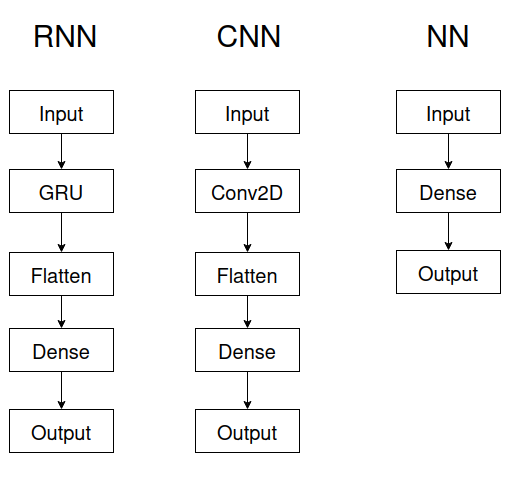
\includegraphics[width=\textwidth]{images/architectures.png}
    \caption[opis dla siatki]{Rysunki poglądowe stworzonych architektur sieci
    głębokich}
    \label{arch}
\end{figure}

% Evaluation metrics: Describe the evaluation metrics you used to 
% measure the performance of your models. Explain why you chose these 
% metrics and how they relate to the research question or problem.
\subsection{Ewaluacja jakości modelu}

Stworzone wytrenowane modele zostały ewaluowane na zbiorze testowym złożonym
z danych meteorologicznych pochodzących ze stycznia z lat 2020 - 2022.
W celu porównania uzyskanych wyników stworzono zestawienia i wykresy pokazujące
korelację, błąd średniokwadratowy oraz błąd bezwzględny poszczególnych modeli.

% Code availability: Consider making your code available to others, 
% and provide a link or repository where readers can access the code 
% you developed. This can facilitate replication of your research and 
% allow others to build upon your work.
\subsection{Dostępność kodu}

Przeprowadzone badania zostały zaimplementowane przy pomocy notatnika Jupyter
\cite{jupyter}, przy pomocy platformy Colab \cite{colab}. Odpowiedni projekt
Jupyter Notebook powinien być dostępny poprzez \url{https://colab.research.google.com/drive/1Fm1UZYe36pVOuCa8jpCKAUoyUJyf3Zmp?usp=sharing}.